% ============================================================================
%  Einsum, Treewidth, and the Convergence Rates of Multiplicative Series
%
%  An exploration companion to
%  "On computing and the complexity of computing higher-order U-statistics,
%   exactly" (Chen, Zhang, Liu).
%
%  Build:  latexmk -pdf main.tex      (or pdflatex; bibtex; pdflatex x2)
%  Figures are produced by the scripts in code/ (run code/run_all.py).
% ============================================================================
\documentclass[11pt]{article}

\usepackage[a4paper, margin=1in]{geometry}
\usepackage{amsmath,amssymb,amsthm,mathtools,bm}
\usepackage{enumitem}
\usepackage{graphicx}
\usepackage{booktabs}
\usepackage{array}
\usepackage[dvipsnames]{xcolor}
\usepackage{tikz}
\usetikzlibrary{arrows.meta, positioning, calc, decorations.pathreplacing}
\usepackage[numbers,sort&compress]{natbib}
\usepackage[colorlinks=true, linkcolor=NavyBlue!70!black,
            citecolor=ForestGreen!60!black, urlcolor=BrickRed!70!black]{hyperref}
\usepackage{cleveref}

% ---- notation mirroring the companion paper --------------------------------
\newcommand{\Einsum}{\textsc{Einsum}}
\newcommand{\tensorcontraction}{\Einsum}
\newcommand{\bbR}{\mathbb{R}}
\newcommand{\bbN}{\mathbb{N}}
\newcommand{\bbZ}{\mathbb{Z}}
\newcommand{\bbX}{\mathbb{X}}
\newcommand{\bbE}{\mathbb{E}}
\newcommand{\calA}{\mathcal{A}}
\newcommand{\calT}{\mathcal{T}}
\newcommand{\calW}{\mathcal{W}}
\newcommand{\calL}{\mathcal{L}}
\newcommand{\calG}{\mathcal{G}}
\newcommand{\calO}{\mathcal{O}}
\newcommand{\bX}{\bm{X}}
\newcommand{\tw}{\mathsf{tw}}
\newcommand{\treewidthp}[1]{\tw(#1)}
\newcommand{\graphform}[1]{G_{#1}}
\newcommand{\ustat}{\mathbb{U}}
\newcommand{\vstat}{\mathbb{V}}
\newcommand{\spec}{\mathrm{spec}}
\newcommand{\rank}{\mathrm{rank}}
\newcommand{\tr}{\operatorname{tr}}
\newcommand{\diam}{\operatorname{diam}}
\newcommand{\sgn}{\operatorname{sgn}}
\newcommand{\eqdef}{\coloneqq}
\newcommand{\less}{\lesssim}
\newcommand{\pressure}{P}
\newcommand{\opteinsum}{\texttt{opt\_einsum}}
\newcommand{\torch}{\texttt{torch.einsum}}
\newcommand{\cotengra}{\texttt{cotengra}}

\theoremstyle{plain}
\newtheorem{theorem}{Theorem}[section]
\newtheorem{proposition}[theorem]{Proposition}
\newtheorem{lemma}[theorem]{Lemma}
\newtheorem{corollary}[theorem]{Corollary}
\theoremstyle{definition}
\newtheorem{definition}[theorem]{Definition}
\newtheorem{example}[theorem]{Example}
\theoremstyle{remark}
\newtheorem{remark}[theorem]{Remark}
\newtheorem{principle}[theorem]{Principle}

\Crefname{principle}{Principle}{Principles}

\title{\bf Einsum, treewidth, and the convergence rates of
       multiplicative series}

\author{Xingyu Chen \and Ruiqi Zhang \and Lin Liu\thanks{%
  Exploration note prepared as a companion to the manuscript
  \emph{``On computing and the complexity of computing higher-order
  $U$-statistics, exactly''}~\citep{chen2024ustats}. Draft for internal
  discussion. Correspondence: \texttt{linliu@sjtu.edu.cn}.}}
\date{\today}

\begin{document}
\maketitle

\begin{abstract}
A surprisingly large family of problems in analysis, dynamics, combinatorics
and probability ask for the exponential growth rate of a \emph{partition
function} $Z_L=\sum_{I}\omega(I)$, where $I$ ranges over admissible
``words'' of length $L$ and the weight $\omega$ is (sub)multiplicative along
the word. The limit $\pressure=\lim_{L}\tfrac1L\log Z_L$ is variously called the
pressure, free energy, growth rate, or a critical exponent, and a recurring
working method of the practitioner is to \emph{conjecture} the rate
$\lambda=e^{\pressure}$ (with a possible power-law correction $L^\theta$),
compute $Z_L$ for growing $L$, and check that, after dividing out the conjecture,
the sequence tends to $1$. Our companion paper observed that a $V$-statistic is
exactly an \Einsum{} (a tensor contraction with no free index) and that its exact
cost is $\Theta(n^{\treewidthp{\graphform{\calA}}+1})$, governed by the treewidth
of a decomposition graph. We observe that the very same einsum/treewidth calculus
governs the transfer-matrix engines that produce $Z_L$, and that the
``decomposable vs.\ entangled'' dichotomy a practitioner runs into is precisely
the dichotomy between \emph{bounded} and \emph{growing} treewidth of the weight's
dependency graph. This yields (i) a clean dictionary between the two worlds;
(ii) a precise version of the ``divide out and check $\to 1$'' heuristic, which
is rigorous whenever the weight compresses into a finite transfer operator and in
which the spectral gap is read off from the \emph{speed} of convergence;
(iii) a structured catalogue of examples spanning both regimes; and (iv) four
worked computations that reproduce known constants
($\varphi$, the hard-square constant, $\dim_H E_2$, and an affinity dimension) and
illustrate each phenomenon. The treewidth bound emerges as a complexity scale for
the numerical engines that mathematicians already use to certify convergence
rates.
\end{abstract}

\tableofcontents

% ===========================================================================
\section{Introduction}
\label{sec:intro}
% ===========================================================================

\subsection{A template that keeps reappearing}

Consider a finite alphabet $[q]=\{1,\dots,q\}$, a set
$\calW_L\subseteq[q]^L$ of \emph{admissible words} of length $L$, and a
nonnegative weight $\omega$ defined on $\calW\eqdef\bigcup_L\calW_L$ that is
\emph{submultiplicative} along concatenation, $\omega(IJ)\le\omega(I)\,\omega(J)$.
The associated \emph{partition function} and \emph{pressure} are
\begin{equation}
\label{eq:template}
   Z_L \;=\; \sum_{I\in\calW_L}\omega(I),
   \qquad
   \pressure \;=\; \lim_{L\to\infty}\frac1L\log Z_L,
   \qquad
   \lambda\;=\;e^{\pressure}.
\end{equation}
The limit exists by Fekete's lemma whenever $\calW$ is closed under concatenation
and $\omega$ is submultiplicative. Depending on the field, $\pressure$ is called the
\emph{topological pressure}, the \emph{free energy}, the \emph{growth rate}, the
\emph{(top) Lyapunov exponent}, or a \emph{critical exponent}; $\lambda$ is a
connective constant, an entropy constant, a Stanley--Wilf limit, a joint spectral
radius, and so on. The entire apparatus of \emph{thermodynamic formalism} and
\emph{transfer operators}~\citep{ruelle2004thermodynamic,parry1990zeta,baladi2000positive}
exists precisely to compute $\pressure$ and its corrections.

The motivation for this note came from a concrete instance in fractal geometry.
For an affine iterated function system with linear parts $T_1,\dots,T_q$, Falconer's
\emph{affinity dimension}~\citep{falconer1988hausdorff} is governed by
\begin{equation}
\label{eq:affinity}
   Z_L(s) \;=\; \sum_{I\in[q]^L}\varphi^s(T_{i_1}T_{i_2}\cdots T_{i_L}),
\end{equation}
where $\varphi^s$ is the singular-value function. The natural complaint is that
\eqref{eq:affinity} has ``no decomposable structure: every factor depends on the
\emph{entire} matrix product''. The question this note grew out of is whether the
einsum/treewidth toolkit of the companion paper~\citep{chen2024ustats} can help
\emph{compute} such series, thereby \emph{assisting} the analytic study of their
convergence and convergence rates, and -- more importantly -- whether
\eqref{eq:template} is a rare shape or a pervasive one. It is pervasive.

\subsection{The practitioner's heuristic}

A working mathematician rarely has $\pressure$ in closed form. Instead one
\emph{conjectures} an asymptotic
\begin{equation}
\label{eq:ansatz}
   Z_L \;\sim\; C\,\lambda^{L}\,L^{\theta}\qquad(L\to\infty),
\end{equation}
computes $Z_L$ for as large an $L$ as the budget allows, and tests the conjecture
by \emph{dividing it out}: the diagnostic ratio
\begin{equation}
\label{eq:divideout}
   \frac{Z_{L+1}/Z_L}{\lambda}\,\Bigl(1+\tfrac1L\Bigr)^{-\theta}\ \longrightarrow\ 1
   \qquad\text{iff the conjecture \eqref{eq:ansatz} is correct.}
\end{equation}
If the ratio settles to $1$ the rate is corroborated; the \emph{speed} at which it
settles, and any systematic drift, expose the subleading exponent $\theta$ and the
spectral gap. The two questions we take up are: \emph{when is this heuristic
rigorous}, and \emph{what does it cost to push $L$ far enough to trust it}?

\subsection{The companion paper, in one paragraph}

\citet{chen2024ustats} study the exact computation of higher-order
$U$- and $V$-statistics. A $V$-statistic with a multiplicatively decomposable
kernel $h(\bm x)=\prod_{k}h_k(\bm x[A_k])$ is, after tensorisation
$T_k(\alpha)=h_k(\bX[\alpha])$, \emph{exactly} an Einstein summation with no output
index,
\begin{equation}
\label{eq:vstat-einsum}
   \vstat(h,\bX)\;=\;\Einsum(\calT,\calA)\;=\;
   \sum_{\alpha\in[n]^m}\ \prod_{k=1}^{K}T_k\bigl(\alpha[A_k]\bigr).
\end{equation}
Its \emph{decomposition graph} $\graphform{\calA}$ has the index set $[m]$ as
vertices and an edge between two indices that co-occur in some $A_k$. The central
complexity result is that evaluating \eqref{eq:vstat-einsum} by the optimal index
elimination costs
\begin{equation}
\label{eq:treewidth-bound}
   \Theta\!\bigl(|\calA|\,n^{\treewidthp{\graphform{\calA}}+1}\bigr),
\end{equation}
where $\treewidthp{\graphform{\calA}}$ is the treewidth of $\graphform{\calA}$; the
optimal pairwise schedules of \opteinsum{}/\torch{} attain the same bound in time
\emph{and} space. The link between contraction cost and treewidth goes back to
\citet{markov2008simulating} in the tensor-network literature and to variable
elimination in graphical models~\citep{lauritzen1988local,bodlaender1993tourist};
finding the optimal order is NP-hard~\citep{arnborg1987complexity}, which is why
practical libraries~\citep{smith2018opt,gray2021hyper} use heuristics.

\subsection{Thesis and contributions}

Our thesis is a single sentence:
\begin{quote}\itshape
the transfer-matrix / finite-lattice engines that mathematicians use to estimate
the rate $\lambda$ in \eqref{eq:template} are themselves \Einsum{} contractions,
and the einsum/treewidth calculus of \eqref{eq:treewidth-bound} both classifies
when the ``divide-out'' heuristic is rigorous and quantifies its cost.
\end{quote}
Concretely:
\begin{enumerate}[leftmargin=2.2em,itemsep=2pt]
\item \textbf{A dictionary} (\Cref{sec:dictionary}) between $U$-statistics and
pressure computations. The growth parameter is the \emph{word length} $L$ (the
number of summation indices), not the alphabet size $q$ (the index range); the
weight's dependency graph $G_L$ grows with $L$, and the relevant quantity is the
\emph{asymptotic treewidth} $\sup_L\treewidthp{G_L}$.

\item \textbf{A structural dichotomy} (\Cref{prop:cost,prop:spectral}):
$Z_L$ is computable in time \emph{polynomial} in $L$ if and only if the family is
\emph{transfer-decomposable} ($\sup_L\treewidthp{G_L}<\infty$), in which case
$Z_L=\langle u,T^Lv\rangle$ for a fixed transfer operator $T$, the pressure is
$\log\rho(T)$, and the divide-out diagnostic \eqref{eq:divideout} converges
\emph{geometrically at the spectral-gap rate}. Otherwise $\treewidthp{G_L}$ grows
and the cost is $q^{\Theta(L)}$ -- the ``everything in one lump'' obstruction of
\eqref{eq:affinity}.

\item \textbf{A catalogue} (\Cref{sec:catalogue}) of more than a dozen example
families across both regimes, each tagged with its structure, its known rate
result, and the role computation plays.

\item \textbf{Four worked computations} (\Cref{sec:experiments}) that we actually
ran (code in \texttt{code/}): the golden-mean shift, hard squares on a strip, the
Hausdorff dimension of the continued-fraction set $E_2$, and an affinity dimension.
They reproduce $\varphi$, the hard-square constant $\kappa=1.50304808\ldots$,
$\dim_H E_2=0.5312805062772\ldots$ to $15$ digits, and an affinity dimension, and
each isolates one phenomenon from the dictionary.
\end{enumerate}

Nothing here competes with the deep analytic machinery of the cited works; the
contribution is a unifying \emph{computational} lens that connects the
practitioner's heuristic, the transfer operator, and the treewidth complexity of
the companion paper.

% ===========================================================================
\section{From a fixed einsum to a growth-indexed family}
\label{sec:dictionary}
% ===========================================================================

\subsection{Growth-indexed einsum families}

In \eqref{eq:vstat-einsum} the \Einsum{} expression is \emph{fixed}: $m$ indices,
each of range $n$. To represent a partition function \eqref{eq:template} we let the
\emph{number of indices grow}. Write the weight of a length-$L$ word as a tensor
network: there are tensors $\calT_L=(T_k)$ and a signature
$\calA_L=(A_k)$ with index set $\{i_1,\dots,i_L\}\cup\{\text{bounded internal
legs}\}$, all index ranges equal to $q$ (or to a fixed internal dimension $d$),
such that
\begin{equation}
\label{eq:ZL-einsum}
   Z_L\;=\;\Einsum(\calT_L,\calA_L)\;=\;\sum_{\alpha}\ \prod_k T_k(\alpha[A_k]).
\end{equation}
The decomposition graph $\graphform{\calA_L}$ now has $\Theta(L)$ vertices.
Applying \eqref{eq:treewidth-bound} verbatim, with the role of the sample size $n$
played by the index range $q$, gives the cost of computing $Z_L$ exactly.

\begin{proposition}[Cost of a growth-indexed family]
\label{prop:cost}
The exact evaluation of $Z_L$ via \eqref{eq:ZL-einsum} by optimal index
elimination costs
$\Theta\!\bigl(|\calA_L|\,q^{\treewidthp{\graphform{\calA_L}}+1}\bigr)$.
In particular, writing $W_L\eqdef\treewidthp{\graphform{\calA_L}}$ and noting
$|\calA_L|=\Theta(L)$ for the chain-type networks below,
\begin{itemize}[leftmargin=1.6em,itemsep=1pt]
\item if $\sup_L W_L=W<\infty$, the cost is $\Theta(L\,q^{W+1})$ -- \emph{polynomial
(indeed linear) in the growth parameter $L$};
\item if $W_L=\Theta(L)$ (e.g.\ $\graphform{\calA_L}=K_L$), the cost is
$q^{\Theta(L)}$ -- \emph{exponential in $L$}.
\end{itemize}
\end{proposition}

\begin{proof}
Immediate from the index-elimination bound of \citet[Prop.~1]{chen2024ustats}
applied to $\calA_L$ with index range $q$, together with the matching lower bound
for optimal pairwise schedules. The two bullets substitute the stated $W_L$.
\end{proof}

The transfer-matrix dimension is exactly $q^{W}$ up to constants: a tree
decomposition of width $W$ carries states indexed by the $\le W{+}1$ live indices
at a bag, i.e.\ $q^{W+1}$ values, and elimination marches a separator of $q^{W}$
states along the chain. This identifies the two folklore cost measures.

\begin{principle}[Decomposable $=$ bounded treewidth]
\label{prin:dichotomy}
``$\omega$ compresses into a finite transfer matrix'' $\iff$
``$\sup_L\treewidthp{\graphform{\calA_L}}<\infty$''. The practitioner's feeling
that a weight is \emph{entangled} (``everything depends on everything'') is the
statement that the treewidth of its dependency graph grows with $L$.
\end{principle}

\subsection{Transfer-decomposable families and the spectral rate}

We make the bounded-treewidth case precise for the linearly ordered (pathwidth-%
bounded) families that cover all our examples; this is the genuine
transfer-matrix setting.

\begin{definition}[Transfer-decomposable family]
\label{def:transfer-decomp}
The family \eqref{eq:ZL-einsum} is \emph{transfer-decomposable of width $W$} if
there is a finite state space $\Sigma$ with $|\Sigma|\le q^{W}$, boundary vectors
$u,v\in\bbR_{\ge0}^{\Sigma}$, and a fixed nonnegative \emph{transfer matrix}
$T\in\bbR_{\ge0}^{\Sigma\times\Sigma}$ such that
\begin{equation}
\label{eq:transfer}
   Z_L \;=\; \langle u,\,T^{L}\,v\rangle\qquad\text{for all }L.
\end{equation}
\end{definition}

Subshifts of finite type, one-dimensional lattice models, strips of any
two-dimensional model, and linear cocycles fed through a \emph{linear} functional
are all of this form; \eqref{eq:transfer} is the einsum
\eqref{eq:ZL-einsum} contracted along the chain, of treewidth $1$ in the index
$i_j$'s after the internal legs of dimension $|\Sigma|$ are absorbed.

\begin{proposition}[Spectral rate and the gap]
\label{prop:spectral}
Let \eqref{eq:transfer} hold with $T$ primitive (irreducible and aperiodic),
Perron eigenvalue $\lambda_1=\rho(T)$, second eigenvalue modulus
$|\lambda_2|<\lambda_1$, and $u,v$ not orthogonal to the corresponding Perron
eigenvectors. Put $\delta\eqdef|\lambda_2|/\lambda_1\in[0,1)$. Then
\begin{enumerate}[label=\textup{(\roman*)},leftmargin=2.2em,itemsep=1pt]
\item $\pressure=\log\lambda_1$, i.e.\ $\lambda=\lambda_1$;
\item $Z_L=c\,\lambda_1^{L}\bigl(1+O(\delta^{L})\bigr)$ with
$c=\langle u,w_R\rangle\langle w_L,v\rangle>0$, where $w_R,w_L$ are the right/left
Perron eigenvectors normalised by $\langle w_L,w_R\rangle=1$;
\item $\dfrac{Z_{L+1}}{Z_L}=\lambda_1\bigl(1+O(\delta^{L})\bigr)$.
\end{enumerate}
\end{proposition}

\begin{proof}
By the Perron--Frobenius theorem $\lambda_1$ is a simple eigenvalue with positive
eigenvectors $w_R,w_L$, and the spectral decomposition reads
$T^{L}=\lambda_1^{L}\,\Pi+R^{L}$, where $\Pi=w_Rw_L^{\!\top}$ is the rank-one Perron
projection and $R=T-\lambda_1\Pi$ has spectral radius $|\lambda_2|$. Hence
$Z_L=\langle u,T^Lv\rangle=\lambda_1^{L}\langle u,w_R\rangle\langle w_L,v\rangle
+\langle u,R^{L}v\rangle$, and $\|R^L\|=O(|\lambda_2|^{L})$ gives
$Z_L=c\lambda_1^{L}(1+O(\delta^{L}))$ with $c>0$ by the non-orthogonality
hypothesis. Statements (i) and (iii) follow by taking logarithms and ratios.
(If $\lambda_2$ sits in a Jordan block of size $b$, the error term gains a
polynomial factor $L^{b-1}$ but the geometric rate $\delta$ is unchanged.)
\end{proof}

\begin{corollary}[The divide-out heuristic is rigorous, and reads off the gap]
\label{cor:divideout}
Under \Cref{prop:spectral}, for a conjectured rate $\lambda^\ast$ the diagnostic
$\rho_L\eqdef Z_{L+1}/Z_L$ satisfies $\rho_L/\lambda^\ast\to1$ if and only if
$\lambda^\ast=\lambda_1$, and then
$\rho_L/\lambda_1-1=O(\delta^{L})$. Consequently the spectral gap
$\delta$ is \emph{identifiable from the speed} at which the divided-out ratio
approaches $1$: a $\log|\rho_L-\lambda_1|$ vs.\ $L$ plot has slope $\log\delta$.
\end{corollary}

\Cref{cor:divideout} is the rigorous heart of the heuristic
\eqref{eq:divideout}: dividing out the rate not only \emph{certifies} $\lambda$ in
the transfer-decomposable regime but \emph{measures} the spectral gap. We verify it
numerically to machine precision in \Cref{sec:exp-golden}.

\begin{remark}[Why a genuine power law $L^\theta$ signals non-decomposability]
\label{rem:powerlaw}
A finite primitive $T$ produces a \emph{pure} geometric correction, not a power
law: in \Cref{prop:spectral} there is no $L^{\theta}$ factor. A true subexponential
factor $L^{\theta}$ in $Z_L$ -- such as the conjectured $c_L\sim A\,\mu^L L^{11/32}$
for two-dimensional self-avoiding walks -- can arise only from an
\emph{infinite-dimensional} transfer operator (continuous spectrum, no gap) or from
\emph{criticality} (the gap $\delta\to1$). The very presence of a power-law
correction is therefore a diagnostic that the problem sits in the entangled column;
this is consistent with every entry of \Cref{tab:catalogue} below.
\end{remark}

\subsection{The dictionary}

\Cref{tab:dictionary} states the correspondence. The single most important row is
the first: the companion paper's \emph{sample size} $n$ plays the role of the
\emph{alphabet/state size} $q$, while the companion paper's \emph{kernel order} $m$
plays the role of the \emph{word length} $L$ that tends to infinity.

\begin{table}[t]
\centering
\renewcommand{\arraystretch}{1.25}
\begin{tabular}{@{}p{0.46\textwidth} p{0.46\textwidth}@{}}
\toprule
\textbf{$U$-statistics / einsum world} & \textbf{Pressure / transfer-operator world}\\
\midrule
sample size $n$ (index range) & alphabet / state size $q$ (index range)\\
kernel order $m$ (\# indices, fixed) & word length $L$ (\# indices, $\to\infty$)\\
$V$-statistic $=\Einsum(\calT,\calA)$, no output & partition function $Z_L$\\
decomposition graph $\graphform{\calA}$ & dependency graph $\graphform{\calA_L}$ of the weight\\
treewidth $\treewidthp{\graphform{\calA}}$ & $\log_q(\text{transfer-matrix dim.})$ $=W_L$\\
index elimination / pairwise schedule & transfer-matrix multiplication / tree DP\\
cost $\Theta(n^{\tw+1})$ & cost $\Theta(L\,q^{W+1})$ (decomposable)\\
sparsification, $U\!\to\!V$ Möbius sum & subleading corrections, boundary terms\\
\bottomrule
\end{tabular}
\caption{The dictionary between the companion paper and the pressure world. The
growth parameter is the number of indices.}
\label{tab:dictionary}
\end{table}

% ===========================================================================
\section{Using computation to support a convergence-rate proof}
\label{sec:methodology}
% ===========================================================================

We separate what is \emph{rigorous} from what is \emph{heuristic}.

\paragraph{Decomposable regime (rigorous).}
When the family is transfer-decomposable, \Cref{prop:spectral} turns the rate into
a finite linear-algebra problem: $\lambda=\rho(T)$ is computed once and for all
from a fixed matrix, and the divide-out diagnostic provably converges at rate
$\delta$. There is no asymptotic guesswork: the rate is \emph{computed}, not
estimated, and certified error bounds follow from rigorous eigenvalue enclosures.
At the analytic end of this regime, the transfer operator is trace-class and one
uses its \emph{spectral determinant} $\det(I-zT)$, whose Taylor coefficients are
cycle sums; these converge \emph{super-exponentially} (factorially) for real-analytic
expanding systems, which is how \citet{jenkinson2018hundred} certify $100$ digits of
$\dim_H E_2$ and \citet{mcmullen1998hausdorff,pollicott2010maximal} compute conformal
dimensions and Lyapunov exponents.

\paragraph{Entangled regime (heuristic, but principled).}
When $\treewidthp{\graphform{\calA_L}}$ grows there is no finite $T$. One then
computes $Z_L$ to the largest feasible $L$ -- where \Cref{prop:cost} says the cost
is $q^{\Theta(L)}$, so the feasible $L$ is set by the affordable treewidth -- and
applies the \emph{ratio method} and \emph{series analysis} (Padé and differential
approximants) of statistical mechanics and enumerative
combinatorics~\citep{guttmann2009polygons,jensen2004enumeration}. This is exactly
the divide-out procedure \eqref{eq:divideout}, now used to \emph{fit} both $\lambda$
and the power-law exponent $\theta$. It is not rigorous, but it is frequently the
\emph{only} route to the conjectured exponent and is the standard practice behind,
e.g., the connective-constant corrections for self-avoiding walks and the
Stanley--Wilf limit of $1324$-avoiding permutations~\citep{conway2018ts}.

\paragraph{What computation contributes to a proof.}
In the decomposable regime, computation \emph{is} the proof: certifying
$\lambda=\rho(T)$ is a finite, checkable calculation. In the entangled regime the
honest statement is that an infinite-dimensional but \emph{low-dimensional-state}
operator often re-emerges -- on a projective space or flag manifold for matrix
cocycles~\citep{falconer1988hausdorff,kaenmaki2004natural,morris2018matrix,
barany2019hausdorff} -- under a \emph{domination/cone} condition, which is the exact
hypothesis that restores a spectral gap and hence rapid, rigorous computation. The
practitioner's intuition that an ``approximate factorisation into independent
parts'' would help is, precisely, the request for a dominated splitting.

% ===========================================================================
\section{A catalogue of examples}
\label{sec:catalogue}
% ===========================================================================

We list example families, grouped by regime. Throughout, ``\textsf{TM}'' marks the
transfer-matrix dimension or state space; ``\textsf{tw}'' marks the asymptotic
treewidth of $\graphform{\calA_L}$.

\subsection{Decomposable: bounded treewidth, rigorous and fast}
\label{sec:cat-decomp}

\begin{enumerate}[leftmargin=1.5em,itemsep=3pt]
\item \textbf{Subshifts of finite type / topological entropy.} $Z_L=$ number of
admissible length-$L$ words $=\mathbf 1^\top A^L\mathbf 1$ for the $0/1$ adjacency
matrix $A$; $\lambda=\rho(A)$, $\pressure=$ topological entropy. \textsf{tw}$=1$. The
golden-mean shift (\Cref{sec:exp-golden}) is the smallest instance.

\item \textbf{One-dimensional statistical mechanics.} $Z_L=\tr(T^L)$ with the
Boltzmann transfer matrix $T$; free energy $=\log\rho(T)$ and correlation length
$=1/\log(\lambda_1/\lambda_2)$ -- \emph{the gap of \Cref{prop:spectral} is a physical
observable}. Ising, Potts, and the hard-hexagon model (Baxter's exact
solution~\citep{baxter1980hard,baxter1982exactly}) live here.

\item \textbf{Strips of two-dimensional models.} On a width-$W$ strip the model is
one-dimensional with $\textsf{TM}=q^{\Theta(W)}$ and \textsf{tw}$=W$: hard
squares~\citep{calkin1998number} (\Cref{sec:exp-hard}), dimers / perfect matchings
(Kasteleyn~\citep{kasteleyn1961statistics}), independent sets, colourings. The
per-site rate converges to the bulk constant as $W\to\infty$; \Cref{prop:cost} makes
the strip width the treewidth dial that trades accuracy against an exponential cost.

\item \textbf{Hausdorff dimension of conformal / cookie-cutter sets.} Bowen's
formula~\citep{bowen1979hausdorff}: $\dim_H=$ the root $s^\ast$ of
$\pressure(s)=0$, where $\pressure(s)$ is the pressure of $-s\log|f'|$. Computed to
extreme precision via transfer operators: the continued-fraction set $E_2$
(\Cref{sec:exp-cf}; \citet{jenkinson2001computing,jenkinson2018hundred}), Julia
sets and Kleinian limit sets~\citep{mcmullen1998hausdorff}.

\item \textbf{Gauss--Kuzmin--Wirsing constant} $\approx0.3036$: the second
eigenvalue of the Gauss-map transfer operator~\citep{wirsing1974gauss} -- literally
the spectral gap $\delta$ of \Cref{prop:spectral} for that operator.

\item \textbf{Large-deviation rate functions for Markov additive functionals.} The
scaled cumulant generating function $\Lambda(k)=\lim_L\frac1L\log\bbE[e^{kS_L}]
=\log\rho(T_k)$ is the pressure of a \emph{tilted} transfer matrix
$T_k$~\citep{dembo1998large}; the Gärtner--Ellis theorem is \Cref{prop:spectral}(i).

\item \textbf{Top Lyapunov exponent of random matrix products}
$\gamma=\lim_L\frac1L\bbE\log\|T_{i_1}\cdots T_{i_L}\|$
\citep{furstenberg1960products}: \emph{non}-decomposable for the norm, but
\citet{pollicott2010maximal} computes it rigorously and rapidly via an analytic
transfer operator on projective space -- the dominated/positive case of
\Cref{sec:methodology}. (See \Cref{sec:exp-mat} for the linear-functional
surrogate, which \emph{is} decomposable.)
\end{enumerate}

\subsection{Entangled: growing treewidth, conjecture-and-verify}
\label{sec:cat-entangled}

\begin{enumerate}[leftmargin=1.5em,itemsep=3pt]
\item \textbf{Affinity dimension of self-affine sets} \eqref{eq:affinity}: the
singular-value function $\varphi^s$ is a \emph{global spectral} functional of the
whole product, so $\graphform{\calA_L}=K_L$ and \textsf{tw}$=L-1$. Rigorous theory
via the matrix/sub-additive pressure and equilibrium states
\citep{falconer1988hausdorff,kaenmaki2004natural,morris2018matrix,barany2019hausdorff};
see \Cref{sec:exp-mat}.

\item \textbf{$\ell^p$ joint spectral radius}
$\rho_p=\lim_L(\sum_{|I|=L}\|T_I\|^p)^{1/(pL)}$~\citep{rota1960note,jungers2009joint}:
the same $K_L$ entanglement as affinity dimension. Sobering honest notes: deciding
$\rho\le1$ is \emph{undecidable}~\citep{blondel2000boundedness}, and the finiteness
conjecture is \emph{false}~\citep{bousch2002asymptotic}. This is the hardest column.

\item \textbf{Self-avoiding walks: connective constant.} $c_L=\#\{\text{SAW of
length }L\}$, $\mu=\lim c_L^{1/L}$; on the honeycomb lattice
$\mu=\sqrt{2+\sqrt2}$~\citep{duminil2012connective}. The self-avoidance constraint is
global, so finite-lattice transfer matrices have \textsf{tw}$=$ strip width and one
pushes $L$ as far as the treewidth budget allows~\citep{jensen2004enumeration}; the
conjectured $c_L\sim A\mu^L L^{11/32}$ in 2D is obtained by dividing out $\mu^L$ and
fitting the power-law exponent~\citep{madras1993self,guttmann2009polygons} --
\emph{exactly} the heuristic \eqref{eq:divideout}, and a power law as in
\Cref{rem:powerlaw}.

\item \textbf{Lattice animals / polyominoes} (growth constant $\approx4.0626$) and
\textbf{pattern-avoiding permutations} (Stanley--Wilf limits, finite by
\citet{marcus2004excluded}; the $1324$ class has only numerical bounds
$\approx11.60$~\citep{conway2018ts}): global constraints, series-analysis exponents.

\item \textbf{Multifractal $L^q$-spectrum} $\tau(q)$ of a self-similar/self-affine
measure, defined through $\sum_I\mu(Q_I)^q$~\citep{falconer1997techniques}:
decomposable for self-similar measures (a scalar potential, \textsf{tw}$=1$),
entangled for genuinely self-affine ones.

\item \textbf{Mahler measure / Lehmer's problem}~\citep{boyd1981speculations}: a
product over conjugates with a different (Diophantine) flavour; included as a
boundary case where the template applies but the transfer structure is subtle.
\end{enumerate}

\begin{table}[t]
\centering
\renewcommand{\arraystretch}{1.2}
\small
\begin{tabular}{@{}lccp{0.34\textwidth}@{}}
\toprule
\textbf{Family} & \textbf{\textsf{tw}$(\graphform{\calA_L})$} & \textbf{Rigorous?}
& \textbf{What computation gives}\\
\midrule
Subshift entropy / 1D stat-mech & $O(1)$ & yes & $\rho(T)$ exactly; gap $=$ corr.\ length\\
2D model on width-$W$ strip & $W$ & yes & bulk rate as $W\!\uparrow$; cost $q^{\Theta(W)}$\\
Conformal Hausdorff dim.\ (Bowen) & $O(1)$ & yes & root of $\pressure(s)=0$; $100+$ digits\\
GKW constant & $O(1)$ & yes & second eigenvalue $=$ gap\\
Lyapunov (proj.\ operator) & $O(1)^\ast$ & yes$^\ast$ & rate under domination\\
\midrule
Affinity dimension & $L-1$ & partial & pressure curve; root $=$ dimension\\
$\ell^p$ joint spectral radius & $L-1$ & no$^{\dagger}$ & estimates; \emph{undecidable} in general\\
SAW connective constant & strip $W$ & partial & $\mu$ and power law by ratio method\\
Lattice animals / permutations & strip $W$ & no & growth constant + exponent (fit)\\
\bottomrule
\end{tabular}
\caption{Catalogue at a glance. ``$\ast$'': the projective transfer operator is
infinite-dimensional but has a fixed low-dimensional \emph{state space} and a gap
under domination. ``$\dagger$'': \citet{blondel2000boundedness,bousch2002asymptotic}.}
\label{tab:catalogue}
\end{table}

% ===========================================================================
\section{Four worked computations}
\label{sec:experiments}
% ===========================================================================

All numbers below were produced by the scripts in \texttt{code/} (run
\texttt{python3 code/run\_all.py}); each reproduces a known constant as a
correctness check.

\subsection{Golden-mean shift: the divide-out diagnostic reads the gap}
\label{sec:exp-golden}

Let $Z_L$ be the number of binary words of length $L$ with no two adjacent $1$s,
the simplest subshift of finite type, with transfer matrix
$T=\bigl(\begin{smallmatrix}1&1\\1&0\end{smallmatrix}\bigr)$, so $Z_L=F_{L+2}$
(Fibonacci) and \textsf{tw}$=1$. The eigenvalues are
$\lambda_1=\varphi=\tfrac{1+\sqrt5}2$ and $\lambda_2=-1/\varphi$, so
\Cref{prop:spectral} predicts $Z_{L+1}/Z_L\to\varphi$ with geometric error at rate
$\delta=|\lambda_2|/\lambda_1=\varphi^{-2}=0.38196601\ldots$ \Cref{fig:golden}
confirms both: the ratio reaches $\varphi=1.6180339887\ldots$, and the
divided-out error $|Z_{L+1}/Z_L-\varphi|$ falls on the line of slope
$\log(\varphi^{-2})$ down to $10^{-15}$. The measured per-step decay is $0.381965$
against the predicted $0.381966$. This is \Cref{cor:divideout} in action: the slope
of the error plot \emph{is} the spectral gap.

\begin{figure}[t]
\centering
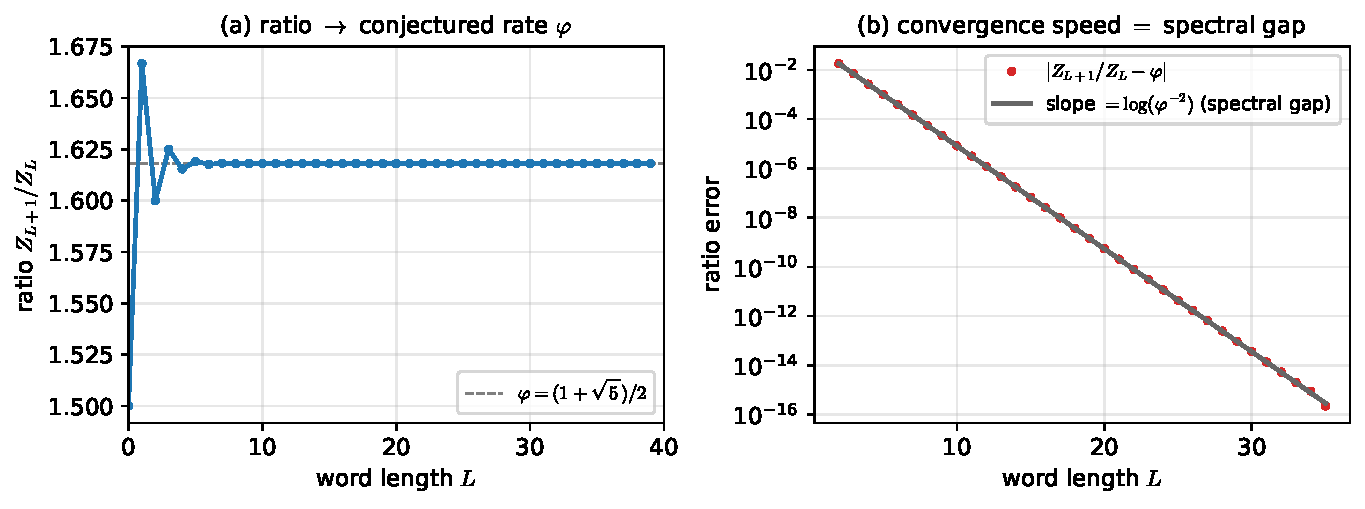
\includegraphics[width=\textwidth]{figures/exp1_golden_mean.pdf}
\caption{Golden-mean shift (decomposable, \textsf{tw}$=1$).
(a) $Z_{L+1}/Z_L\to\varphi$. (b) the divided-out error decays geometrically at
exactly the spectral-gap rate $\varphi^{-2}$, illustrating \Cref{cor:divideout}:
dividing out the rate \emph{measures} the gap.}
\label{fig:golden}
\end{figure}

\subsection{Hard squares on a strip: treewidth is the accuracy/cost dial}
\label{sec:exp-hard}

The hard-square model (no two horizontally or vertically adjacent occupied sites)
on a width-$W$ strip is one-dimensional with transfer matrix $M_W$ indexed by the
independent sets of the path $P_W$; its dimension is $F_{W+2}\sim\varphi^{W}$,
precisely the $q^{\textsf{tw}}$ of \Cref{prop:cost} with \textsf{tw}$=W$. The
per-site rate $\lambda_1(M_W)^{1/W}$ and the incremental ratio
$\lambda_1(M_W)/\lambda_1(M_{W-1})$ both converge to the hard-square constant
$\kappa=1.5030480824753\ldots$~\citep{calkin1998number,baxter1982exactly}, the
latter \emph{geometrically} (\Cref{fig:hard}): at $W=14$ it already matches $\kappa$
to $13$ digits. The point is structural: wider strips give better estimates of the
bulk rate, but the transfer-matrix dimension -- and hence the cost, by
\Cref{prop:cost} -- grows like $\varphi^{W}$. \emph{The feasible treewidth caps the
attainable accuracy}, which is exactly the message the companion bound sends to the
enumeration engines of \Cref{sec:cat-entangled}.

\begin{figure}[t]
\centering
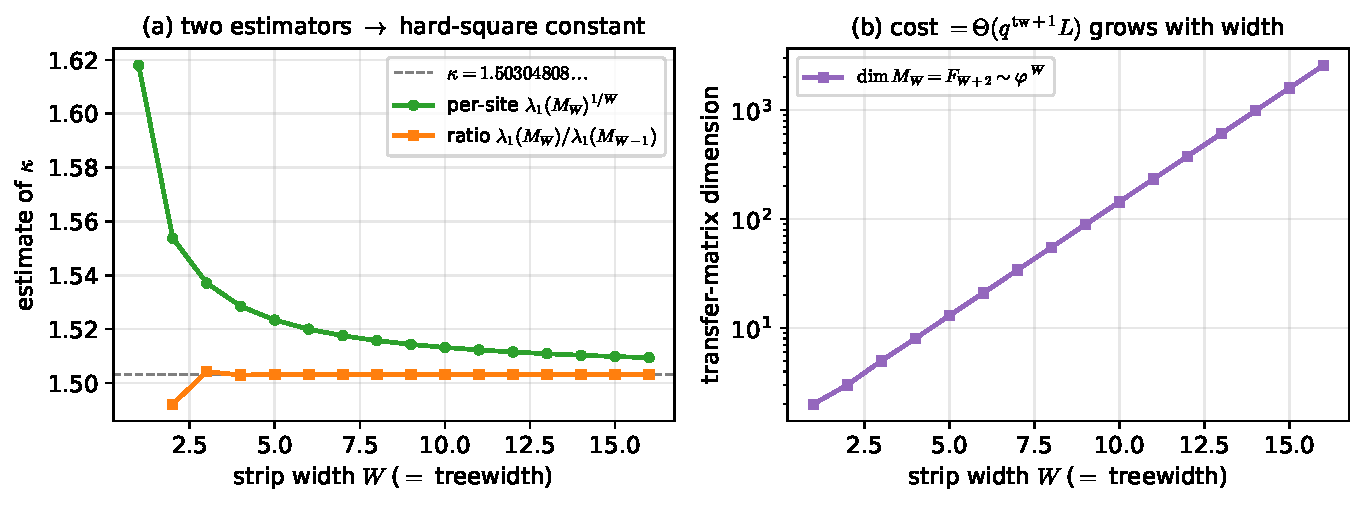
\includegraphics[width=\textwidth]{figures/exp2_hard_squares.pdf}
\caption{Hard squares on a width-$W$ strip (\textsf{tw}$=W$).
(a) two estimators converge to $\kappa$; the ratio estimator is geometric.
(b) the transfer-matrix dimension $=F_{W+2}\sim\varphi^{W}$ is the
$q^{\textsf{tw}}$ cost of \Cref{prop:cost}.}
\label{fig:hard}
\end{figure}

\subsection{Continued-fraction dimension $E_2$: divide out $\to1$ at the right $s$}
\label{sec:exp-cf}

Let $E_2$ be the set of continued fractions $[0;a_1,a_2,\dots]$ with all digits in
$\{1,2\}$. Its Hausdorff dimension $s^\ast$ is the Bowen root of the pressure of the
transfer operator
$(\calL_sf)(x)=\sum_{a\in\{1,2\}}(a+x)^{-2s}f(1/(a+x))$, i.e.\ the $s$ with leading
eigenvalue $\lambda(s)=1$. The weight $\varphi_I(x)=|D(\psi_{a_1}\!\circ\cdots\circ
\psi_{a_L})(x)|^s$ is multiplicative along the word by the chain rule, so the
operator has a \emph{fixed} finite state space even though the alphabet is infinite
in the unrestricted Gauss map. Two cross-checked computations (\Cref{fig:cf}):
\begin{itemize}[leftmargin=1.6em,itemsep=1pt]
\item \textbf{operator route.} A Chebyshev collocation of $\calL_s$ on $N{+}1$ nodes
(independent of word length) plus a root-find in $s$ gives, at $N=16$,
$s^\ast=0.5312805062772$, matching the reference
value~\citep{jenkinson2018hundred} to $\approx15$ digits; convergence in $N$ is
spectral (\Cref{fig:cf}(a)). The operator's spectral gap is $\delta\approx0.31$.
\item \textbf{word route.} Enumerating all $2^L$ words and forming $Z_L(s)$, the
divided-out ratio $Z_{L+1}(s)/Z_L(s)$ tends to $1$ \emph{iff} $s=s^\ast$: at
$s^\ast$ it is $1.000000$, while at $s^\ast\mp0.03$ it locks onto $1.0387$ and
$0.9628$ (\Cref{fig:cf}(b)). This is the cleanest possible realisation of ``set $s$
to the conjectured dimension and check the ratio $\to1$''.
\end{itemize}
This is the prototypical case in which \emph{computation assists a proof}: the
dimension is a transcendental constant known only through such transfer-operator
calculations.

\begin{figure}[t]
\centering
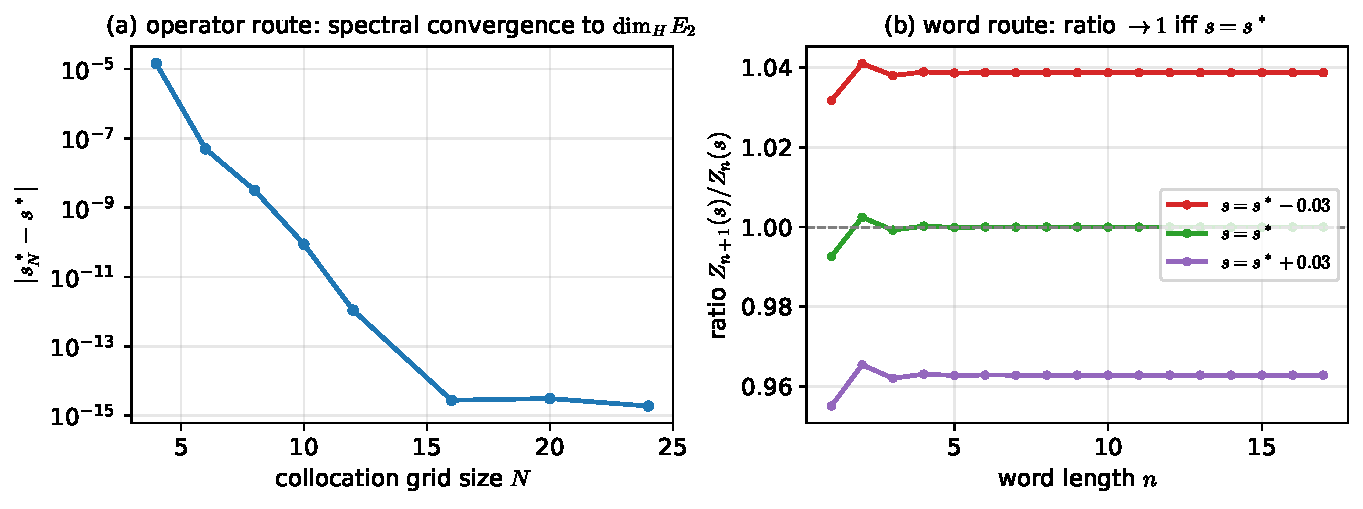
\includegraphics[width=\textwidth]{figures/exp3_continued_fraction.pdf}
\caption{Hausdorff dimension of the continued-fraction set $E_2$ (decomposable via
a fixed-state transfer operator). (a) spectral convergence of the operator estimate
to $\dim_H E_2$. (b) the word-enumeration ratio $\to1$ iff $s=s^\ast$.}
\label{fig:cf}
\end{figure}

\subsection{Matrix products: the entangled case and when it collapses}
\label{sec:exp-mat}

Finally we treat the motivating family \eqref{eq:affinity} on explicit $2\times2$
matrices. The singular-value functional couples all $L$ indices, so the
decomposition graph is $K_L$ (\textsf{tw}$=L-1$): the only exact route is brute
force over $q^L$ words. Two phenomena (\Cref{fig:mat}):

\textbf{(a) Collapse of the rate onto a decomposable surrogate.} Replacing the
operator norm by the \emph{linear} functional trace makes the weight multiplicative:
$\sum_{|I|=L}\tr(T_I)=\tr(S^L)$ with $S=\sum_iT_i$, whose dependency graph is the
path $P_L$ (\textsf{tw}$=1$, cost $O(L)$). For \emph{nonnegative} matrices
Perron--Frobenius forces the two pressures to coincide,
$\lim_L\frac1L\log\sum_{|I|=L}\|T_I\|=\log\rho(S)$, so the cheap decomposable
surrogate \emph{proves} the rate that brute force only estimates. Numerically the
surrogate gives $\log\rho(S)=0.114986731574$ in closed form, and the brute-force
norm-sum (graph $K_L$) drifts toward the same value (\Cref{fig:mat}(a)). For
\emph{signed} matrices the coincidence fails -- our example gives norm-rate
$0.149$ against $\log\rho(S)=-0.153$ -- which is the honest boundary where the
trace surrogate is invalid and one needs the projective/flag-manifold operator of
\Cref{sec:methodology}.

\textbf{(b) Affinity dimension as a pressure root.} With $\varphi^s=\sigma_1^s$ for
$s\le1$ and $\sigma_1\sigma_2^{s-1}$ for $1\le s\le2$, the affinity dimension is the
root of $\pressure(s)=0$. The brute-force pressure curve $\pressure_L(s)$ at $L=18$
yields $s^\ast\approx1.089$ (\Cref{fig:mat}(b)). The endpoint $s=2$ is a free
validation: there $\varphi^2=|\det|$ is fully multiplicative
(\textsf{tw}$=0$), so $Z_L(2)=(\,|\det T_1|+|\det T_2|\,)^L$ in closed form, and the
brute-force value $\frac1L\log Z_L(2)=-1.195674002$ matches the closed form to all
printed digits. The decomposition $\varphi^s=|\det|^{\,s-1}\sigma_1^{\,2-s}$
($1\le s\le2$) exhibits the split cleanly: the determinant factor is a
fully decomposable scalar potential, and only the $\sigma_1^{\,2-s}$ factor is
entangled.

\begin{figure}[t]
\centering
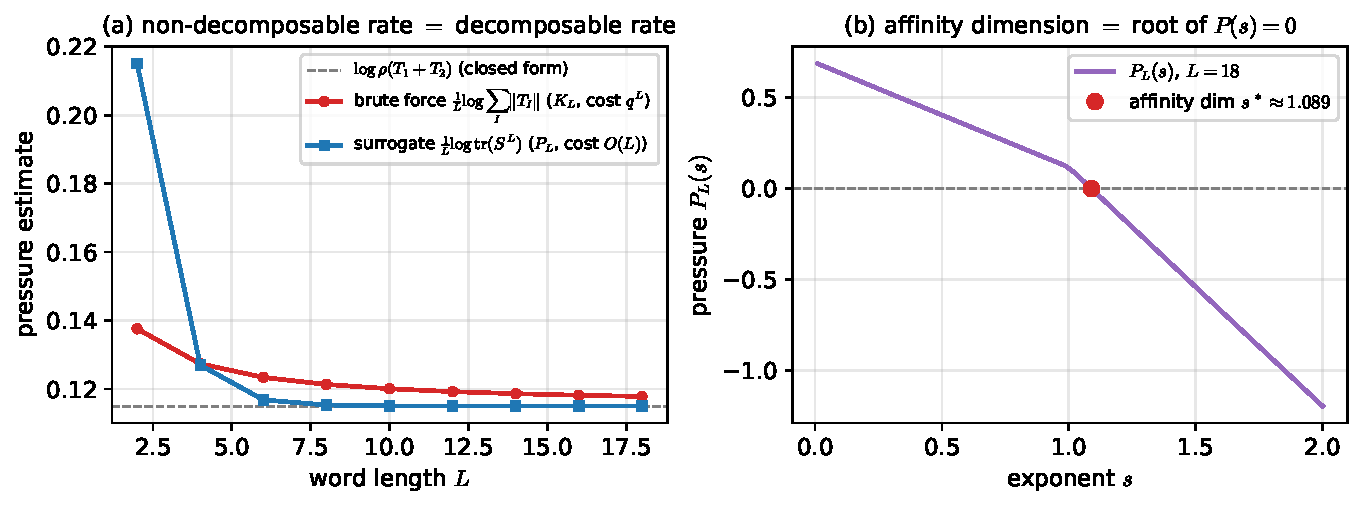
\includegraphics[width=\textwidth]{figures/exp4_matrix_products.pdf}
\caption{Matrix products (entangled, $\graphform{\calA_L}=K_L$).
(a) the non-decomposable norm-sum rate and the decomposable trace surrogate share
the limit $\log\rho(T_1{+}T_2)$ for nonnegative matrices. (b) affinity dimension as
the root of the pressure $\pressure(s)=0$; $s=2$ is a closed-form validation.}
\label{fig:mat}
\end{figure}

% ===========================================================================
\section{Discussion}
\label{sec:discussion}
% ===========================================================================

\paragraph{What the treewidth theorem contributes.}
The catalogue's entangled column is computed, in practice, by transfer-matrix /
finite-lattice engines: SAW and lattice-animal enumeration, dimer counting, hard-%
particle partition functions. \Cref{prop:cost} says these are \Einsum{}
contractions whose decomposition graph is a strip of width $W$, so the companion
bound $\Theta(q^{\,\textsf{tw}+1})$ \emph{is} the complexity scale of the engines
that certify convergence rates: how wide a strip (how large an $L$, how accurate a
rate) is reachable is dictated by the treewidth, which is the message of the hard-%
square experiment. The companion paper therefore speaks not only to $U$-statistics
but to a much wider class of ``numerically assisted'' convergence-rate problems.

\paragraph{Limits.}
Finding the optimal elimination order is NP-hard~\citep{arnborg1987complexity}; the
entangled column has genuine obstructions, including undecidability of the joint
spectral radius~\citep{blondel2000boundedness} and the failure of the finiteness
conjecture~\citep{bousch2002asymptotic}; and the ratio method is heuristic outside
the decomposable regime. The power-law diagnostic of \Cref{rem:powerlaw} is a useful
sanity check: a clean geometric correction is the fingerprint of a finite transfer
matrix.

\paragraph{Outlook.}
Three directions seem worthwhile. (i) \emph{Off-the-shelf pressure engines}: the
contraction-path optimisers \opteinsum{}/\cotengra{}~\citep{smith2018opt,gray2021hyper}
already solve the scheduling half of \Cref{prop:cost}; wrapping them as a generic
``$Z_L$-to-$\pressure$'' tool with automatic gap estimation would directly serve the
practitioners of \Cref{sec:catalogue}. (ii) \emph{Automatic detection of
transfer-decomposability}: deciding whether a weight admits a width-$W$ carrier is a
treewidth question on $\graphform{\calA_L}$, amenable to the same heuristics.
(iii) \emph{Back to $U$-statistics}: degenerate or growing-order $U$-statistics, where
the kernel order $m$ scales with $n$, are themselves growth-indexed families, and the
pressure viewpoint may illuminate the asymptotics of their variance and limiting
distribution.

\paragraph{Reproducibility.}
The four experiments live in \texttt{code/} (\texttt{exp1}--\texttt{exp4},
driver \texttt{run\_all.py}) and regenerate the figures in \texttt{figures/}; each
prints the constant it reproduces as a self-check.

\small
\bibliographystyle{plainnat}
\bibliography{references}

\end{document}
